\section{Arhitectura DVM versiunea 1}

Prima versiune a mediatorului cu valori implicite expune către echipamentul de control \gls{sdn} modelul informațional simplificat pentru microunde, care a fost folosit în cea de-a doua demonstraţie de concept efectuată de proiectul \gls{wt} din \gls{onf} \cite{stancu2016default}.

Implementarea acestuia este una simplă și modulară, bazată pe soluţia \textit{OpenYuma}, oferind câte o funcție cu apel invers pentru fiecare atribut din modelele \gls{yang} expuse, indiferent de natura lor (parametri de configurare sau de stare). În aceste funcții se stabileşte valoare atributului respectiv, care este returnată unui client \gls{netconf}. Excepţia de la această regulă este dată de câteva atribute ale căror valori sunt definite într-un fişier de configurare folosit de către mediator. Dezavantajul acestei abordări este că dacă un dezvoltator de aplicații are nevoie de o altă valoare a unui atribut care nu face parte din acest fişier de configurare, va trebui să o modifice în funcţia asociată parametrului respectiv și apoi să recompileze codul asociat modului de server care conţine acel parametru și apoi să încarce din nou acel modul în server.

O imagine de ansamblu a arhitecturii primii versiuni a \gls{dvm} este ilustrată în Figura \ref{fig:dvm_v01_architecture}. Acesta se bazează pe un fişier de configurare ce conţine câțiva parametri importanţi din punctul de vedere al aplicațiilor \gls{sdn}. Aceștia sunt: (i) numele echipamentului de rețea - \textit{Network Element Name} și (ii) un identificator unic folosit pentru fiecare legătură radio - \textit{Radio Signal ID}.

\begin{figure}[h]
	\centering
	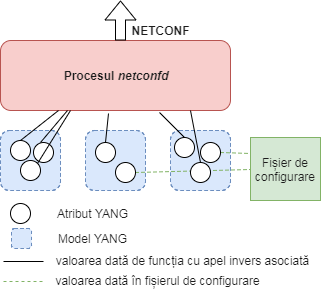
\includegraphics{dvm_v01_architecture}
	\caption{Arhitectura primei versiuni a DVM \cite{stancu2016default}.}
	\label{fig:dvm_v01_architecture}
\end{figure}

Aceşti parametri sunt importanţi pentru aplicații deoarece cu ajutorul lor se pot identifica în mod unic dispozitivele din rețea. Prin pregătirea mai multor fişiere de configurare se pot simula mai multe elemente de rețea, fără a fi nevoie de recompilarea simulatorului. Astfel, vor rula mai multe instanţe ale \gls{dvm}, fiecare având propriul fişier de configurare ce conţine un alt nume pentru dispozitiv și alte identificatoare pentru legăturile radio.

În această arhitectură, \gls{dvm} este configurat să trimită și notificări \gls{netconf} fictive către utilizatorii care s-au abonat la primirea acestora. Fişierul de configurare conţine astfel și o valoare numerică reprezentând numărul de secunde dintre două notificări fictive consecutive. Dacă această valoare este mai mare decât zero, se vor trimite notificări fictive la intervalul de timp specificat. Altfel, dacă valoarea este zero, \gls{dvm} nu va trimite astfel de mesaje \gls{netconf}.